\documentclass[]{article}
\usepackage{lmodern}
\usepackage{amssymb,amsmath}
\usepackage{ifxetex,ifluatex}
\usepackage{fixltx2e} % provides \textsubscript
\ifnum 0\ifxetex 1\fi\ifluatex 1\fi=0 % if pdftex
  \usepackage[T1]{fontenc}
  \usepackage[utf8]{inputenc}
\else % if luatex or xelatex
  \ifxetex
    \usepackage{mathspec}
  \else
    \usepackage{fontspec}
  \fi
  \defaultfontfeatures{Ligatures=TeX,Scale=MatchLowercase}
\fi
% use upquote if available, for straight quotes in verbatim environments
\IfFileExists{upquote.sty}{\usepackage{upquote}}{}
% use microtype if available
\IfFileExists{microtype.sty}{%
\usepackage{microtype}
\UseMicrotypeSet[protrusion]{basicmath} % disable protrusion for tt fonts
}{}
\usepackage[margin=1in]{geometry}
\usepackage{hyperref}
\hypersetup{unicode=true,
            pdftitle={DATA 609 - Homework 1},
            pdfauthor={Joshua Sturm},
            pdfborder={0 0 0},
            breaklinks=true}
\urlstyle{same}  % don't use monospace font for urls
\usepackage{longtable,booktabs}
\usepackage{graphicx,grffile}
\makeatletter
\def\maxwidth{\ifdim\Gin@nat@width>\linewidth\linewidth\else\Gin@nat@width\fi}
\def\maxheight{\ifdim\Gin@nat@height>\textheight\textheight\else\Gin@nat@height\fi}
\makeatother
% Scale images if necessary, so that they will not overflow the page
% margins by default, and it is still possible to overwrite the defaults
% using explicit options in \includegraphics[width, height, ...]{}
\setkeys{Gin}{width=\maxwidth,height=\maxheight,keepaspectratio}
\IfFileExists{parskip.sty}{%
\usepackage{parskip}
}{% else
\setlength{\parindent}{0pt}
\setlength{\parskip}{6pt plus 2pt minus 1pt}
}
\setlength{\emergencystretch}{3em}  % prevent overfull lines
\providecommand{\tightlist}{%
  \setlength{\itemsep}{0pt}\setlength{\parskip}{0pt}}
\setcounter{secnumdepth}{0}
% Redefines (sub)paragraphs to behave more like sections
\ifx\paragraph\undefined\else
\let\oldparagraph\paragraph
\renewcommand{\paragraph}[1]{\oldparagraph{#1}\mbox{}}
\fi
\ifx\subparagraph\undefined\else
\let\oldsubparagraph\subparagraph
\renewcommand{\subparagraph}[1]{\oldsubparagraph{#1}\mbox{}}
\fi

%%% Use protect on footnotes to avoid problems with footnotes in titles
\let\rmarkdownfootnote\footnote%
\def\footnote{\protect\rmarkdownfootnote}

%%% Change title format to be more compact
\usepackage{titling}

% Create subtitle command for use in maketitle
\newcommand{\subtitle}[1]{
  \posttitle{
    \begin{center}\large#1\end{center}
    }
}

\setlength{\droptitle}{-2em}

  \title{DATA 609 - Homework 1}
    \pretitle{\vspace{\droptitle}\centering\huge}
  \posttitle{\par}
    \author{Joshua Sturm}
    \preauthor{\centering\large\emph}
  \postauthor{\par}
      \predate{\centering\large\emph}
  \postdate{\par}
    \date{September 7, 2018}


\begin{document}
\maketitle

\hypertarget{chapter-1-problems}{%
\section{Chapter 1 problems}\label{chapter-1-problems}}

\hypertarget{page-8-exercise-10}{%
\subsection{1 (Page 8, exercise \#10)}\label{page-8-exercise-10}}

Your grandparents have an annuity. The value of the annuity increases
each month by an automatic deposit of 1\% interest on the previous
month's balance. Your grandparents withdraw \$1000 at the beginning of
each month for living expenses. Currently, they have \$50,000 in the
annuity. Model the annuity with a dynamical system. Will the annuity run
out of money? When? Hint: What value will \(a_n\) have when the annuity
is depleted?

\hypertarget{solution}{%
\subsubsection{1 Solution}\label{solution}}

\indent The change in value from month to month is given by
\begin{align*}
    \Delta a_n &= a_{n + 1} - a_n \\
    \Delta a_n &= 0.01 \times a_{n - 1} - 1000
\end{align*}

Solving for \(a_{n + 1}\) gives us the difference equation
\begin{align*}
    a_{n + 1} &= a_n + 0.01 \times a_n - 1000 \\
    a_0 &= 50000
\end{align*}

We can write a function to calculate the value each month until it's
depleted.

\begin{verbatim}
## [1] 49500
## [1] 48995
## [1] 48484.95
## [1] 47969.8
## [1] 47449.5
## [1] 46923.99
## [1] 46393.23
## [1] 45857.16
## [1] 45315.74
## [1] 44768.89
## [1] 44216.58
## [1] 43658.75
## [1] 43095.34
## [1] 42526.29
## [1] 41951.55
## [1] 41371.07
## [1] 40784.78
## [1] 40192.63
## [1] 39594.55
## [1] 38990.5
## [1] 38380.4
## [1] 37764.21
## [1] 37141.85
## [1] 36513.27
## [1] 35878.4
## [1] 35237.18
## [1] 34589.56
## [1] 33935.45
## [1] 33274.81
## [1] 32607.55
## [1] 31933.63
## [1] 31252.97
## [1] 30565.5
## [1] 29871.15
## [1] 29169.86
## [1] 28461.56
## [1] 27746.18
## [1] 27023.64
## [1] 26293.87
## [1] 25556.81
## [1] 24812.38
## [1] 24060.51
## [1] 23301.11
## [1] 22534.12
## [1] 21759.46
## [1] 20977.06
## [1] 20186.83
## [1] 19388.7
## [1] 18582.58
## [1] 17768.41
## [1] 16946.09
## [1] 16115.55
## [1] 15276.71
## [1] 14429.48
## [1] 13573.77
## [1] 12709.51
## [1] 11836.6
## [1] 10954.97
## [1] 10064.52
## [1] 9165.165
## [1] 8256.817
## [1] 7339.385
## [1] 6412.779
## [1] 5476.907
## [1] 4531.676
## [1] 3576.992
## [1] 2612.762
## [1] 1638.89
## [1] 655.2788
## [1] -338.1684
## [1] 70
\end{verbatim}

The annuity would lose all value in the 70th month.

Graph of the annuity's value over time:

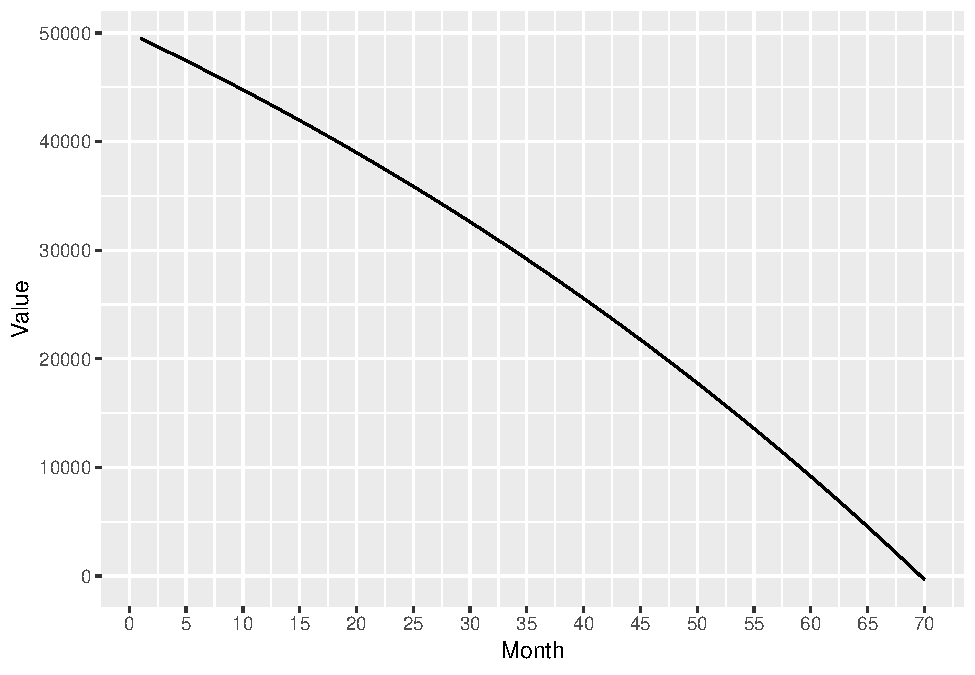
\includegraphics{DATA_609_Homework_1_files/figure-latex/annuity-graph-1.pdf}

\hypertarget{page-17-exercise-9}{%
\subsection{2 (Page 17, exercise \#9)}\label{page-17-exercise-9}}

The data in the accompanying table show the speed \(n\) (in increments
of 5 mph) of an automobile and the associated distance \(a_n\) in feet
required to stop it once the brakes are applied. For instance, \(n = 6\)
(representing \(6 \times 5 = 30\) mph) requires a stopping distance of
\(a_6 = 47\) ft.

\begin{enumerate}
\def\labelenumi{\alph{enumi}.}
\item
  Calculate and plot the change \(\Delta a_n\) versus \(n\). Does the
  graph reasonably approximate a linear relationship?
\item
  Based on your conclusions in part (a), find a difference equation
  model for the stopping distance data. Test your model by plotting the
  errors in the predicted values against \(n\). Discuss the
  appropriateness of the model.
\end{enumerate}

\begin{longtable}[]{@{}lrrrrrrrrrrrrrrrr@{}}
\toprule
\endhead
n & 1 & 2 & 3 & 4 & 5 & 6 & 7 & 8 & 9 & 10 & 11 & 12 & 13 & 14 & 15 &
16\tabularnewline
an & 3 & 6 & 11 & 21 & 32 & 47 & 65 & 87 & 112 & 140 & 171 & 204 & 241 &
282 & 325 & 376\tabularnewline
\bottomrule
\end{longtable}

\hypertarget{solution-1}{%
\subsubsection{2 Solution}\label{solution-1}}

\hypertarget{a}{%
\paragraph{2a}\label{a}}

\(\Delta a_n = a_{n + 1} - a_n\)

\begin{longtable}[]{@{}lrrrrrrrrrrrrrrrr@{}}
\toprule
\endhead
n & 1 & 2 & 3 & 4 & 5 & 6 & 7 & 8 & 9 & 10 & 11 & 12 & 13 & 14 & 15 &
16\tabularnewline
an & 3 & 6 & 11 & 21 & 32 & 47 & 65 & 87 & 112 & 140 & 171 & 204 & 241 &
282 & 325 & 376\tabularnewline
delta & 3 & 5 & 10 & 11 & 15 & 18 & 22 & 25 & 28 & 31 & 33 & 37 & 41 &
43 & 51 & NA\tabularnewline
\bottomrule
\end{longtable}

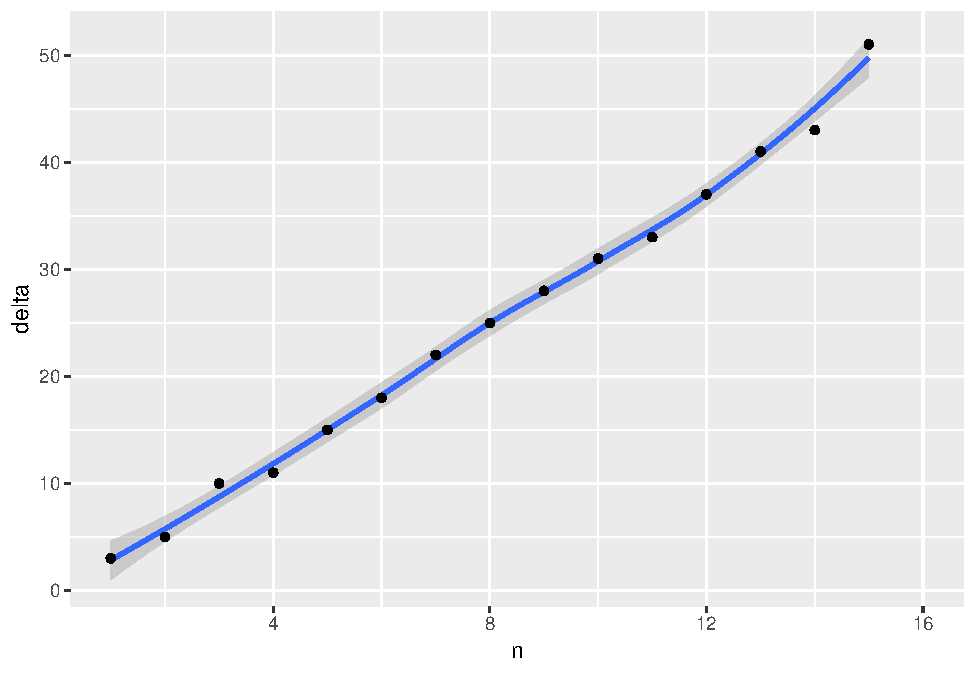
\includegraphics{DATA_609_Homework_1_files/figure-latex/2a-1.pdf}

The graph indicates a linear relationship between \(n\) and
\(\Delta a_n\).

\hypertarget{b}{%
\paragraph{2b}\label{b}}

Our difference equation model is given by \begin{equation*}
a_{n + 1} = a_b + \Delta_n
\end{equation*}

We can find \(\Delta_n\) by taking the slope of the graph, since we've
already determined that there is a linear relationship between \(n\) and
\(\Delta a_n\).

The slope of the graph is 3.246, and the intercept is -1.105.

Our difference equation is now \begin{equation*}
a_{n + 1} = a_n + 3.246\times n - 1.105
\end{equation*}

\begin{verbatim}
##     n  an delta predicted  error
## 1   1   3     3     3.000  0.000
## 2   2   6     5     5.141  0.859
## 3   3  11    10    11.387 -0.387
## 4   4  21    11    19.633  1.367
## 5   5  32    15    32.879 -0.879
## 6   6  47    18    47.125 -0.125
## 7   7  65    22    65.371 -0.371
## 8   8  87    25    86.617  0.383
## 9   9 112    28   111.863  0.137
## 10 10 140    31   140.109 -0.109
## 11 11 171    33   171.355 -0.355
## 12 12 204    37   205.601 -1.601
## 13 13 241    41   241.847 -0.847
## 14 14 282    43   282.093 -0.093
## 15 15 325    51   326.339 -1.339
## 16 16 376    NA   372.585  3.415
\end{verbatim}

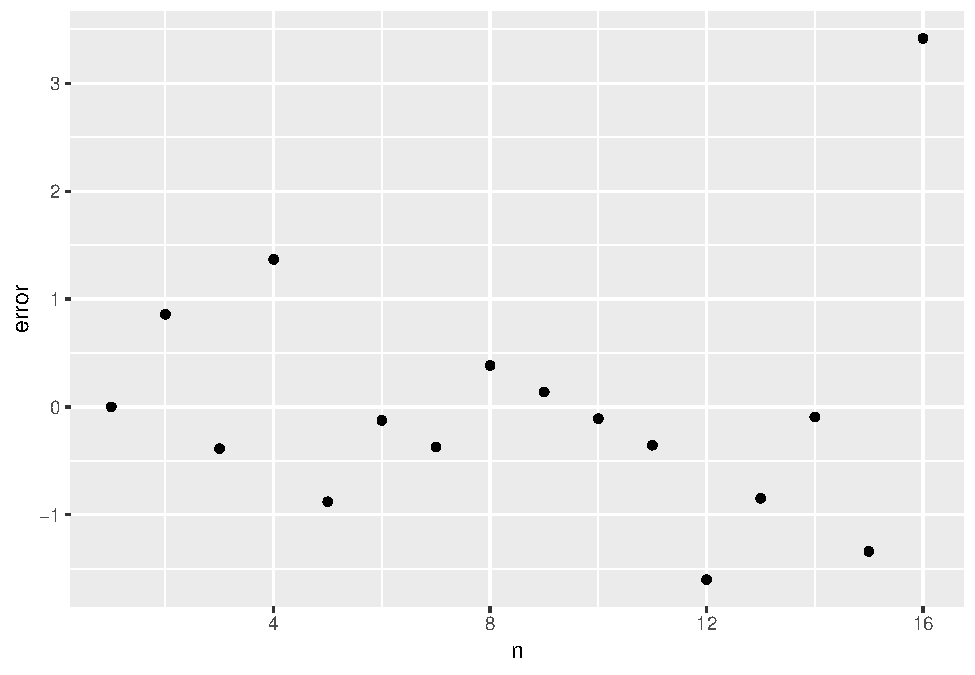
\includegraphics{DATA_609_Homework_1_files/figure-latex/unnamed-chunk-3-1.pdf}

Since the errors do not appear to be normally distributed, one can
conclude that this model would not be appropriate to estimate the
stopping distance.

\hypertarget{page-34-exercise-13}{%
\subsection{3 (Page 34, exercise \#13)}\label{page-34-exercise-13}}

Consider the spreading of a rumor through a company of 1000 employees,
all working in the same building. We assume that the spreading of a
rumor is similar to the spreading of a contagious disease (see Example
3, Section 1.2) in that the number of people hearing the rumor each day
is proportional to the product of the number who have heard the rumor
previously and the number who have not heard the rumor. This is given by
\begin{equation*}
r_{n + 1} = r_n + kr_n(1000 - r_n)
\end{equation*} where \(k\) is a parameter that depends on how fast the
rumor spreads and \(n\) is the number of days. Assume \(k = 0.001\) and
further assume that four people initially have heard the rumor. How soon
will all 1000 employees have heard the rumor?

\hypertarget{solution-2}{%
\subsubsection{3 Solution}\label{solution-2}}

We are given \(r_0 = 4\) and \(k = 0.001\).

\begin{verbatim}
##    Day     Number
## 1    0    4.00000
## 2    1    7.98400
## 3    2   15.90426
## 4    3   31.55557
## 5    4   62.11538
## 6    5  120.37244
## 7    6  226.25535
## 8    7  401.31922
## 9    8  641.58132
## 10   9  871.53605
## 11  10  983.49701
## 12  11  999.72765
## 13  12  999.99993
## 14  13 1000.00000
## 15  14 1000.00000
\end{verbatim}

After 12 days, the rumour will have spread to all employees throughout
the office.

\hypertarget{page-55-exercise-6}{%
\subsection{4 (Page 55, exercise \#6)}\label{page-55-exercise-6}}

An economist is interested in the variation of the price of a single
product. It is observed that a high price for the product in the market
attracts more suppliers. However, increasing the quantity of the product
supplied tends to drive the price down. Over time, there is an
interaction between price and supply. The economist has proposed the
following model, where \(P_n\) represents the price of the product at
year \(n\), and \(Q_n\) represents the quantity. Find the equilibrium
values for this system.

\begin{align*}
P_{n+1} &= P_n - 0.1(Q_n - 500) \\
Q_{n+1} &= Q_n + 0.2(P_n - 100)
\end{align*}

\begin{enumerate}
\def\labelenumi{\alph{enumi}.}
\item
  Does the model make sense intuitively? What is the significance of the
  constants 100 and 500? Explain the significance of the signs of the
  constants 0:1 and 0.2.
\item
  Test the initial conditions in the following table and predict the
  long-term behavior.
\end{enumerate}

\begin{longtable}[]{@{}lll@{}}
\toprule
NA & Price & Quantity\tabularnewline
\midrule
\endhead
Case A & 100 & 500\tabularnewline
Case B & 200 & 500\tabularnewline
Case C & 100 & 600\tabularnewline
Case D & 100 & 400\tabularnewline
\bottomrule
\end{longtable}

\hypertarget{a-solution}{%
\subsubsection{4a Solution}\label{a-solution}}

The equilibrium is when we have \(P = P_{n+1} = P_n\) and
\(Q = Q_{n+1} = Q_n\) simultaneously. After solving the system of
equations, we find the equilibrium when \(P = 100\) and \(Q = 500\).

These are the equilibrium values. The model makes sense, as it
illustrates the relationship between quantity and price. As supply
increases, price will drop; conversely, when supply decreases, price
will rise.

The sign of the coefficients explain the relationship. For example, in
the first equation, the model estimates that the price decreases by
\$0.10 for every additional unit added to the market.

\hypertarget{b-solution}{%
\subsubsection{4b Solution}\label{b-solution}}

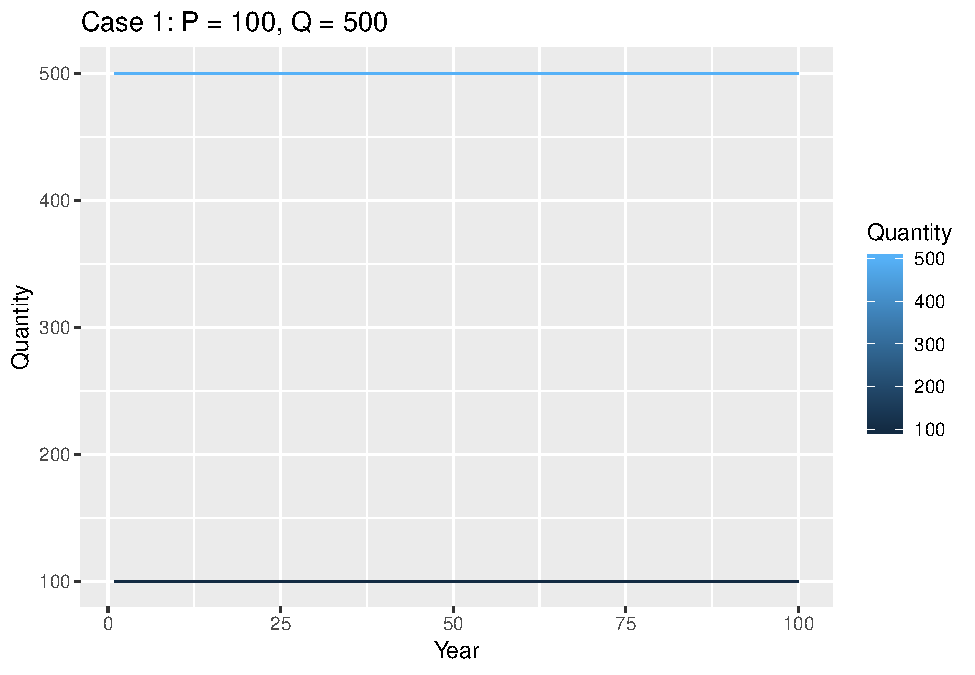
\includegraphics{DATA_609_Homework_1_files/figure-latex/unnamed-chunk-7-1.pdf}

There is no change, since both variables are at their equilibrium.

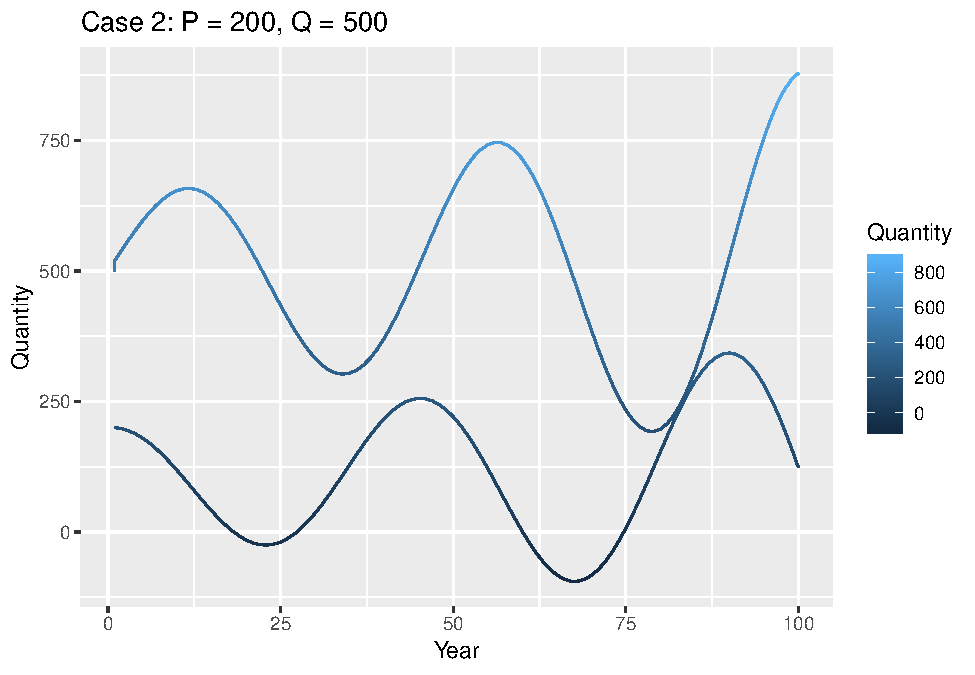
\includegraphics{DATA_609_Homework_1_files/figure-latex/unnamed-chunk-8-1.pdf}

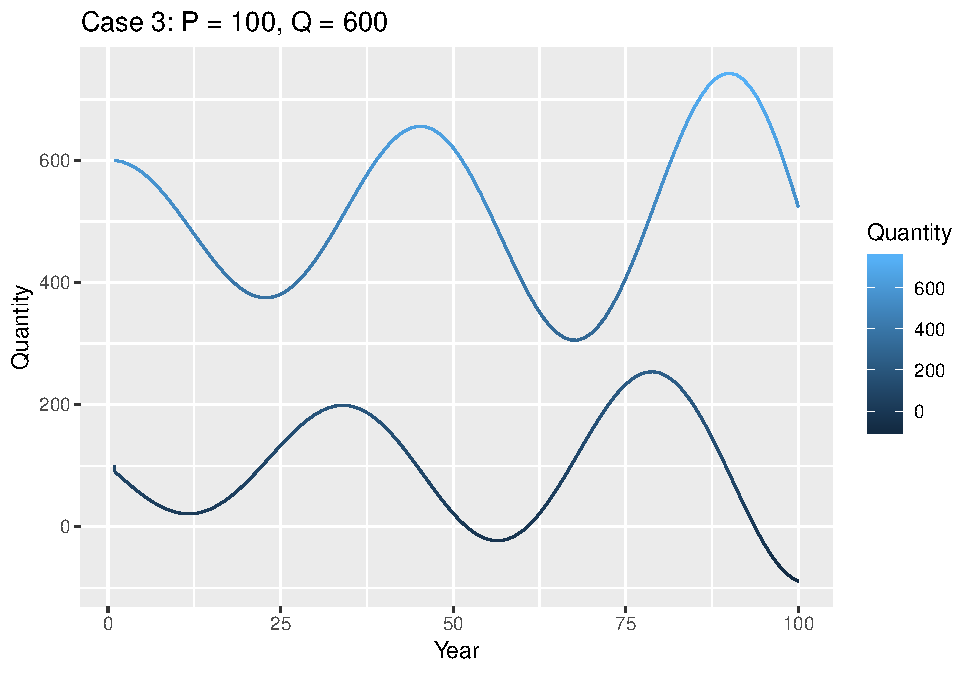
\includegraphics{DATA_609_Homework_1_files/figure-latex/unnamed-chunk-9-1.pdf}

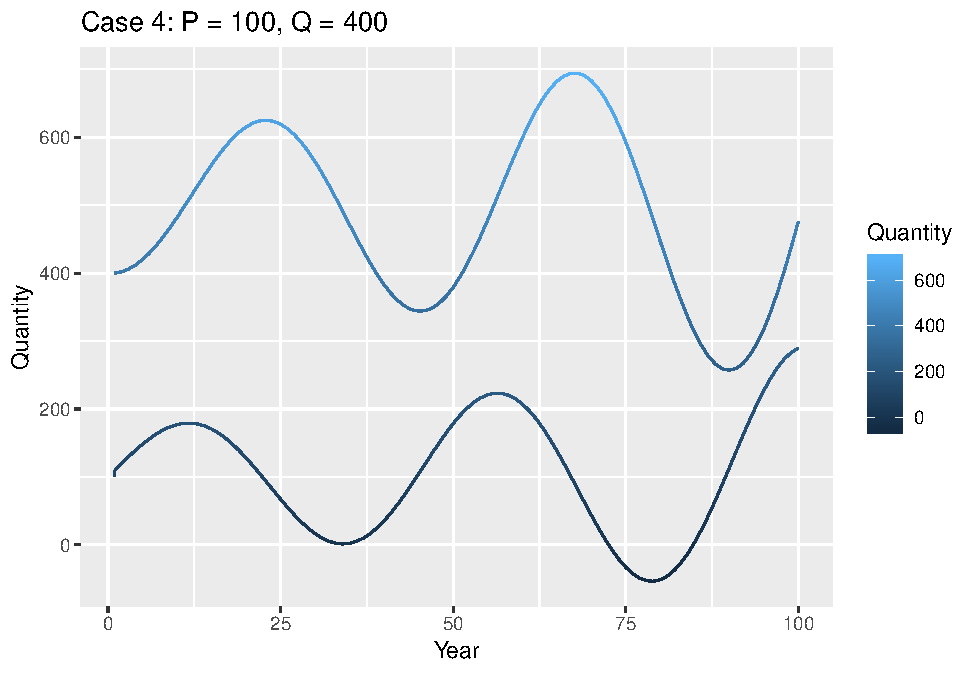
\includegraphics{DATA_609_Homework_1_files/figure-latex/unnamed-chunk-10-1.pdf}


\end{document}
